\documentclass{article}
\usepackage{spconf,amsmath,graphicx}
\usepackage{mathtools}
\usepackage{xfrac}
\usepackage{amsfonts}
\usepackage{amsthm}
\usepackage{subfig}
\usepackage{hyperref}
\usepackage{xcolor}
\usepackage{times}
\usepackage{float}
\usepackage{algorithm,algorithmic}


\newtheorem{theorem}{Theorem}
\newtheorem{lemma}{Lemma}

\renewcommand{\algorithmicrequire}{\textbf{Input:}}
\renewcommand{\algorithmicensure}{\textbf{Output:}}

\allowdisplaybreaks

\title{Bayesian neural networks for sparse coding}

\name{Danil Kuzin$^{\dagger}$ \qquad Olga Isupova$^{\star}$ \qquad Lyudmila Mihaylova$^{\dagger}$}

\address{$^{\dagger}$ Department of Automatic Control and Systems Engineering,\\
University of Sheffield, Sheffield S1 3JD, UK\\
e-mail: dkuzin1@sheffield.ac.uk; l.s.mihaylova@sheffield.ac.uk.\\
$^{\star}$ Department of Engineering Science,\\
University of Oxford, Oxford OX1 2JD, UK\\
e-mail: olga.isupova@eng.ox.ac.uk}

\begin{document}

\maketitle

\begin{abstract}
  Deep learning is actively used in the area of sparse coding. In current deep sparse coding methods uncertainty of predictions is rarely estimated, thus providing the results that lack the quantitative justification. Bayesian learning provides the way to estimate the uncertainty of predictions in neural networks (NNs) by imposing the prior distributions on weights, propagating the resulting uncertainty through the layers and computing the posterior distributions of predictions. We propose a novel method of propagating the uncertainty through the sparsity-promoiting layers of NNs for the first time. We design a Bayesian Learned Iterative Shrinkage-Thresholding network (Bayes\textsc{lista}). An efficient posterior inference algorithm based on probabilistic backpropagation is developed. Experiments on sparse coding show that the proposed framework provides both accurate predictions and sensible estimates of uncertainty in these predictions.
\end{abstract}

\begin{keywords}
sparse coding, Bayesian neural networks, uncertainty estimation, compressive sensing
\end{keywords}

\section{Introduction}
\label{sec:intro}

  The idea of Bayesian learning in neural networks (NNs)~\cite{neal2012bayesian} has recently gained an attention with the development of distributed approximate inference techniques~\cite{li2015stochastic, hoffman2013stochastic} and general boost in popularity of deep learning. In addition to predictions, Bayesian learning naturally provides the uncertainty estimates of these predictions. These uncertainty estimates are vital, e.g., in spheres that affect people's health, such as self-driving cars or medicine.

  Recently several techniques~\cite{ranganath2015deep, gal2016dropout} have been proposed to handle specific types of NNs with efficient Bayesian inference. For example, feed-forward networks with the rectified linear unit nonlinearity~\cite{hernandez2015probabilistic}, networks with discrete distributions~\cite{soudry2014expectation}, recurrent networks~\cite{mcdermott2017bayesian}.

  In this paper, we consider the area of sparse coding. The sparse coding problem can be viewed as a linear regression problem with the additional assumption that the majority of the basis representation coefficients should be zeros. This sparsity assumption may be represented as $l1$ penalty~\cite{tibshirani1996regression}, or, in Bayesian interpretation, as a prior that has a sharp peak at zero~\cite{tipping2001sparse}. One of the modern approaches for sparse coding utilises NNs with the soft-thresholding nonlinearity~\cite{gregor2010learning, sprechmann2015learning}. Sparse coding is widely used in different applications, such as compressive sensing~\cite{candes2008introduction}, image and video processing~\cite{mairal2014sparse, wang2015deep}, neuroscience~\cite{baillet1997bayesian, jas2017learning}.

  A novel method to propagate uncertainty through the soft-thresholding nonlinearity is proposed in this paper. At every layer the current distribution of the target vector is approximated with a spike and slab distribution~\cite{mitchell1988bayesian}, which represents the probabilities of each variable being zero, or Gaussian-distributed. Using the proposed method of uncertainty propagation, the gradients of the logarithms of normalisation constants are derived, which can be used to update a weight distribution. A novel Bayesian NN for sparse coding is designed utilising both the proposed method of uncertainty propagation and Bayesian inference algorithm.

  The main contributions of this paper are: (\textit{i}) for the first time a method for uncertainty propagation through the soft-thresholding nonlinearity is proposed for a Bayesian NN; (\textit{ii}) an efficient posterior inference algorithm for weights and outputs of NNs with the soft-thresholding nonlinearity is developed; (\textit{iii}) a novel Bayesian NN for sparse coding is designed.

% The rest of the paper is organised as follows. A novel Bayesian neural network is introduced in Section~\ref{sec:bayesian_lista}. The proposed forward uncertainty propagation and probabilistic backpropagation methods are given in Sections~\ref{sec:fprop} and~\ref{sec:backpropagation}. Section~\ref{sec:experiments} provides the experimental results and Section~\ref{sec:conclusions} concludes the paper.

\section{Neural networks for sparse coding}
  \label{sec:bayesian_lista}
 % This section first reviews existing NNs for sparse coding and then introduces the novel Bayesian NN.
 This section presents background knowledge about NNs for sparse coding and then describes the novel Bayesian NN.

\subsection{Frequentist neural networks}
\label{subsec:nn_sc}
  The NN approach to sparse coding is based on earlier Iterative Shrinkage and Thresholding Algorithm (\textsc{ista}) \cite{daubechies2004iterative}. It addresses the sparse coding problem as the linear regression problem with the $l1$ penalty that promotes sparsity. For the linear regression model with observations $\mathbf{y} \in \mathbb{R}^K$, the design matrix $\mathbf{X} \in \mathbb{R}^{K \times D}$, and the sparse unknown vector of weights $\boldsymbol\beta \in \mathbb{R}^D$, \textsc{ista} minimises
  \begin{equation}
  \label{eq:regression_problem}
  ||\mathbf{X}\boldsymbol\beta - \mathbf{y}||_2^2 + \alpha ||\boldsymbol\beta||_1 \, \text{w.r.t.} \,\boldsymbol\beta,
  \end{equation}
  where $\alpha$ is a regularisation parameter.

  At every iteration $l$, \textsc{ista} obtains the new estimate $\widehat{\boldsymbol\beta}_l$ of the target vector $\boldsymbol\beta$ as the linear transformation $\mathbf{b} = \mathbf{W}\mathbf{y} + \mathbf{S}\widehat{\boldsymbol\beta}_{l-1}$ propagated through the soft-thresholding function %$h_\lambda(\cdot)$
  \begin{equation}
  h_\lambda(\mathbf{b}) = \text{sgn}(\mathbf{b}) \max(|\mathbf{b}| - \lambda, 0),
  \end{equation}
  where $\lambda$ is a shrinkage parameter.
  In \textsc{ista}, weights $\mathbf{W}$ and $\mathbf{S}$ of the linear transformation are assumed fixed.

  In contrast to \textsc{ista}, Learned \textsc{ista} (\textsc{lista}) \cite{gregor2010learning} learns the values of matrices $\mathbf{W}$ and $\mathbf{S}$ based on a set of pairs $\{\mathbf{Y}, \mathbf{B}\}=\{\mathbf{y}^{(n)}, \boldsymbol\beta^{(n)}\}_{n=1}^N$, where $N$ is the number of these pairs. To achieve this, \textsc{ista} is limited with the fixed amount of iterations $L$ and interpreted as a recurrent NN: every iteration $l$ of \textsc{ista} corresponds to the layer $l$ of \textsc{lista}. A vector $\boldsymbol\beta$ for an observation~$\mathbf{y}$ is predicted by Algorithm~\ref{alg:lista}.

  \begin{algorithm}[t]
    \caption{\textsc{lista} forward propagation}
    \label{alg:lista}
    \begin{algorithmic}[1]
      \REQUIRE observations $\mathbf{y}$, weights $\mathbf{W}, \mathbf{S}$, number of layers $L$
      \STATE Dense layer $\mathbf{b} \gets \mathbf{W}\mathbf{y}$ \label{eq:first_layer}
      \STATE Soft-thresholding nonlinearity~$\widehat{\boldsymbol\beta}_0 \gets h_\lambda(\mathbf{b})$ \label{eq:thr_first}
      \FOR{$l=1$ \TO $L$}
        \STATE Dense layer $\mathbf{c}_l \gets \mathbf{b} + \mathbf{S}\widehat{\boldsymbol\beta}_{l-1}$ \label{eq:l_dense_layer}
        \STATE Soft-thresholding nonlinearity $\widehat{\boldsymbol\beta}_{l} \gets h_\lambda(\mathbf{c}_l)$ \label{eq:l_thr}
      \ENDFOR
      \RETURN $\widehat{\boldsymbol\beta} \gets \widehat{\boldsymbol\beta}_{L}$
    \end{algorithmic}
  \end{algorithm}

 % In \textsc{lista}, matrices $\mathbf{W}$ and $\mathbf{S}$ are the parameters that are initialised as in the \textsc{ista} and then updated with the backpropagation algorithm. Vectors $\mathbf{c}_l$ and $\mathbf{b}$ are auxiliary vectors that describe forward propagation.

  \subsection{Bayes\textsc{lista}}
  \label{subsec:bayesian_lista}
  This section introduces the proposed Bayesian version of \textsc{lista} (Bayes\textsc{lista}). The prior distributions are imposed on the unknown weights
  \begin{equation}
  \label{eq:ws}
  \begin{split}
  p(\mathbf{W}) &= \prod_{d=1}^D\prod_{k=1}^K \mathcal{N}(w_{dk} ; 0, \eta^{-1}), \\
  p(\mathbf{S}) &= \prod_{d'=1}^D\prod_{d''=1}^D \mathcal{N}(s_{d'd''} ; 0, \eta^{-1}),
  \end{split}
  \end{equation}
  where $\eta$ is the precision of the Gaussian distribution.

  For every layer $l$ of Bayes\textsc{lista}, $\widehat{\boldsymbol\beta}_{l}$ is assumed to have the spike and slab distribution with the spike probability $\boldsymbol\omega$, the slab mean $\mathbf{m}$, and the slab variance $\mathbf{v}$
  \begin{equation}
  [\widehat{\boldsymbol\beta}_{l}]_d \sim \omega_d \delta_0 + (1 - \omega_d)\mathcal{N}(m_d, v_d),
  \end{equation}
  where $\delta_0$ is the delta-function that represents a spike, $[\cdot]_d$ denotes the $d$-th component of a vector. Section \ref{sec:fprop} shows that the output of the next layer $\widehat{\boldsymbol\beta}_{l+1}$ can be approximated with the spike and slab distribution and, therefore, the output of the Bayes\textsc{lista} network $\widehat{\boldsymbol\beta}$ has the spike and slab distribution.

  To introduce the uncertainty of predictions, we assume that the true $\boldsymbol\beta$ is an output $f(\mathbf{y} ; \mathbf{S}, \mathbf{W}, \lambda)$ of the Bayes\textsc{lista} network corrupted by the additive Gaussian zero-mean noise with the precision~$\gamma$. Then the likelihood of $\mathbf{B}$ is defined as
  \begin{equation}
  \label{eq:likelihood}
  \begin{split}
  p(\mathbf{B}| \mathbf{Y}, &\mathbf{W}, \mathbf{S}, \gamma, \lambda) \\
  = &\prod_{n=1}^N\prod_{d=1}^D\mathcal{N}\left(\beta_d^{(n)}; [f(\mathbf{y} ; \mathbf{S}, \mathbf{W}, \lambda)]_d, \gamma^{-1}\right)
 \end{split}
  \end{equation}
  Gamma prior distributions with parameters~$a^{\cdot}$ and~$b^{\cdot}$ are specified on the introduced Gaussian precisions
  \begin{equation}
  \label{eq:gamma_eta}
  p(\gamma) = \text{Gam}\left(\gamma; a^{\gamma}, b^{\gamma}\right), \qquad
  p(\eta) = \text{Gam}\left(\eta; 	a^{\eta}, b^{\eta}\right)
  \end{equation}

  The posterior distribution is then
  \begin{equation}
  \label{eq:posterior}
  \begin{split}
  p(\mathbf{W}, \mathbf{S}, &\gamma, \eta | \mathbf{B}, \mathbf{Y}, \lambda) \\
  = &\frac{p(\mathbf{B} | \mathbf{Y}, \mathbf{W},  \mathbf{S}, \gamma, \lambda) p(\mathbf{W} | \eta )p(\mathbf{S} | \eta) p(\eta) p(\gamma)}{p(\mathbf{B} | \mathbf{Y}, \lambda)}
  \end{split}
  \end{equation}
  The shrinkage parameter $\lambda$ is a hyperparameter of the model.

  \section{Uncertainty propagation through soft-thresholding}
  \label{sec:fprop}
  This section describes modification of \textsc{lista} forward propagation (Algorithm~\ref{alg:lista}) to include probability distributions of the random variables introduced in section~\ref{subsec:bayesian_lista}.

  \subsection{Initialisation}
  \label{subsec:forward_init}
  At step \ref{eq:first_layer} of \textsc{lista} (Algorithm~\ref{alg:lista}) the matrix $\mathbf{W}$ consists of Gaussian-distributed components $w_{dk} \sim \mathcal{N}(m^w_{dk}, v^w_{dk})$, and $\mathbf{y}$ is a deterministic vector. Then the output $\mathbf{b}$ is a vector of Gaussian-distributed components $b_d \sim \mathcal{N}(m^b_d, v^b_d)$, where $m^b_d = \sum_{k=1}^Ky_k m^w_{dk}$, and $v^b_d = \sum_{k=1}^Ky_k^2v^w_{dk}$.
%  \begin{equation}
%  \label{eq:matrix_vector_product}
%  m^b_d = \sum_{k=1}^Ky_k m^w_{dk}, \qquad
%  v^b_d = \sum_{k=1}^Ky_k^2v^w_{dk}.
%  \end{equation}

  At step~\ref{eq:thr_first} of \textsc{lista} (Algorithm~\ref{alg:lista}) the Gaussian vector $\mathbf{b}$ is taken as an input of the soft-thresholding function. When a Gaussian random variable $x \sim \mathcal{N}(x; m, v)$ is propagated through the soft-thresholding function $x^* = h_{\lambda}(x)$, the probability mass of the resulting random variable $x^*$ is split into two parts. The values of $x$ from the interval $[-\lambda, \lambda]$ are converted to~$0$ by the soft-thresholding operator. Therefore, the probability mass of the original distribution that lies in $[-\lambda, \lambda]$ is squeezed into the probability of $x^*$ being zero. The values of $x$ from outside of the $[-\lambda, \lambda]$ interval are shifted towards~$0$. The distribution of $x^* \neq 0$ then represents the tails of the original Gaussian distribution. The distribution of $x^*$ can be then parametrised by the probability of being zero, $\omega^*$, the mean $m^*$ and the variance $v^*$ of the truncated Gaussian distribution.
%  \begin{lemma}[Propagation of a Gaussian variable through soft-thresholding]
%  \label{thm:soft_thresholding}
%  The distribution of $x^*$ can be parametrised by the probability of being zero, $\omega^*$, the mean $m^*$ and the variance $v^*$ of the truncated Gaussian distribution.
%  \end{lemma}
 %Based on the results of Lemma~\ref{thm:soft_thresholding},
 Therefore, we approximate the distribution of $\widehat{\boldsymbol\beta}_0$ at step~\ref{eq:thr_first} with a spike and slab distribution with parameters: the spike probability $\omega^*$, the slab mean $m^*$ and variance $v^*$.

  \subsection{Main layers}
  At step \ref{eq:l_dense_layer} of \textsc{lista} (Algorithm~\ref{alg:lista}) the vector $\mathbf{b}$ and matrix $\mathbf{S}$ consist of Gaussian components: $b_d \sim \mathcal{N}(m^b_d, v^b_d)$, $s_{d'd''} \sim \mathcal{N}(m^s_{d'd''}, v^s_{d'd''})$, and $\widehat{\boldsymbol\beta}_{l-1}$ is a vector of the spike and slab random variables: $[\widehat{\beta}_{l-1}]_d \sim \omega_d \delta_0 + (1 - \omega_d)\mathcal{N}(m_d, v_d)$.

 It can be shown that the expected value and variance of a spike and slab distributed variable $\xi$ with the probability of spike $\omega$, the slab mean $m$ and slab variance $v$ are:
   \begin{equation}
   \label{eq:spsl_moments}
  \mathbb{E}\xi = (1-\omega)m, \qquad \operatorname{Var}\xi = (1-\omega)(v + \omega m^2).
  \end{equation}

 It can also be shown that if components of the matrix $\mathbf{S}$ and vector $\widehat{\boldsymbol\beta}_{l-1}$ are mutually independent then the components $[ \mathbf{e}_l ]_d$ of their product $\mathbf{e}_l = \mathbf{S} \widehat{\boldsymbol\beta}_{l-1}$ have the marginal mean and variances:
  \begin{subequations}
  \label{eq:e_moments}
  \begin{align}
  m^e_{d} \stackrel{\text{def}}{=} &\mathbb{E}[ \mathbf{e}_l ]_d = \sum_{d'=1}^D m^s_{dd'}(1-\omega_{d'})m_{d'}, \\
   \begin{split}
  v^e_{d} \stackrel{\text{def}}{=} &\operatorname{Var}[ \mathbf{e}_l ]_d = \sum_{d'=1}^D [(m^s_{dd'})^2(1-\omega_{d'})^2v_{d'} \\
   + &(1-\omega_{d'})^2(m_{d'})^2v^s_{dd'} + v^s_{dd'}(1-\omega_{d'})^2v_{d'}].
   \end{split}
   \end{align}
  \end{subequations}
According to the Central Limit Theorem $[ \mathbf{e}_l ]_d$ can be approximated as a Gaussian-distributed variable when $D$ is sufficiently large. The parameters of this Gaussian distribution are the marginal mean and variance given in~(\ref{eq:e_moments}).

%  In order to determine the distribution of the output $\mathbf{c}_l$ we first formulate two lemmas.
%
%%  \begin{lemma}[Moments of a spike and slab distribution]
%%  \label{thm:moments_spsl}
%%  Let a random variable $\xi$ have a spike and slab distribution with the probability of spike $\omega$, the slab mean $m$ and slab variance $v$. Then its moments are
%%  \begin{equation}
%%  \mathbb{E}\xi = (1-\omega)m, \qquad \operatorname{Var}\xi = (1-\omega)(v + \omega m^2)
%%  \end{equation}
%%  \end{lemma}
%
%  \begin{lemma}[Product of a Gaussian matrix and a spike and slab vector]
%    \label{thm:matrix_vector}
%  Let $\mathbf{S} \in \mathbb{R}^{D \times D}$ be a matrix of independent Gaussian-distributed random variables: $s_{d'd''} \sim \mathcal{N}(m^s_{d'd''}, v^s_{d'd''})$, and $\widehat{\boldsymbol\beta }\in \mathbb{R}^D$ be a vector with spike-and-slab-distributed variables: $\widehat{\beta}_d \sim \omega_d \delta_0 + (1 - \omega_d)\mathcal{N}(m_d, v_d)$. The components of the matrix $\mathbf{S}$ and the vector $\widehat{\boldsymbol\beta}$ are mutually independent. Let $\mathbf{e} \in \mathbb{R}^{D}$ denote the product $\mathbf{S} \widehat{\boldsymbol\beta}$. Then the marginal mean and variance of the elements $e_d$ of the vector $\mathbf{e}$ are
%  \begin{subequations}
%  \begin{align}
%   \mathbb{E}e_d &= \sum_{d'=1}^D m^s_{dd'}(1-\omega_{d'})m_{d'}, \\
%   \begin{split}
%   \operatorname{Var}e_d &= \sum_{d'=1}^D [(m^s_{dd'})^2(1-\omega_{d'})^2v_{d'} + (1-\omega_{d'})^2(m_{d'})^2v^s_{dd'} + v^s_{dd'}(1-\omega_{d'})^2v_{d'}].
%   \end{split}
%   \end{align}
%  \end{subequations}
%   \end{lemma}
%
%  The proofs of Lemmas~\ref{thm:moments_spsl} and~\ref{thm:matrix_vector} are given in the supplementary materials.
%
%  Let $\mathbf{e}_l$ denote the product $\mathbf{S}\widehat{\boldsymbol\beta}_{l-1}$ at step \ref{eq:l_dense_layer} of \textsc{lista}. We assume that $\mathbf{S}$ and $\widehat{\boldsymbol\beta}_{l-1}$ are mutually independent. Then according to the Central Limit Theorem $[ \mathbf{e}_l ]_d$ can be approximated as a Gaussian-distributed variable when $D$ is sufficiently large. The parameters of the of the approximating Gaussian distribution are set to the marginal mean and variance given in Lemma~\ref{thm:matrix_vector}. The supplementary materials provide a discussion of the quality of this approximation.

  The output $\mathbf{c}_l$ at step \ref{eq:l_dense_layer} is then represented as a sum of two Gaussian-distributed vectors: $\mathbf{b}$ and~$\mathbf{e}_l$, i.e. it is a Gaussian-distributed vector with components $c_{d} \sim \mathcal{N}(m^c_{d}, v^c_{d})$, where $m^c_{d} = m^b_{d} + m^e_{d}$ and $v^c_{d} = v^b_{d} + v^e_{d}$.
%  \begin{equation}
%  \label{eq:sum_vectors}
%  m^c_{d} = m^b_{d} + m^e_{d}, \qquad
%  v^c_{d} = v^b_{d} + v^e_{d}.
%  \end{equation}


  Then $\widehat{\boldsymbol\beta}_{l}$ at step \ref{eq:l_thr} of \textsc{lista} (Algorithm~\ref{alg:lista}) is the result of soft-thresholding of a Gaussian variable, which is approximated with the spike and slab distribution,  similar to step \ref{eq:thr_first} (section~\ref{subsec:forward_init}).
  Thus, all the steps of Bayes\textsc{lista} are covered and distributions for outputs of these steps are derived.

  \section{Backpropagation}
  \label{sec:backpropagation}

  The exact intractable posterior (\ref{eq:posterior}) is approximated with a factorised distribution
  \begin{align}
  q(&\mathbf{W}, \mathbf{S}, \gamma, \eta) = \prod_{d=1}^D\prod_{k=1}^K \mathcal{N}(w_{dk} ; m^w_{dk}, v^w_{dk}) \text{Gam}(\gamma; a^\gamma, b^\gamma)\nonumber\\
  \label{eq:approximating_dsitribution}
  &\times\prod_{d'=1}^D\prod_{d''=1}^D \mathcal{N}(s_{d'd''} ; m^s_{d'd''}, v^s_{d'd''}) \text{Gam}(\eta; a^\eta, b^\eta).
  \end{align}

  Parameters of approximating distributions are updated with the assumed density filtering (ADF) and expectation propagation (EP) algorithms derived on the derivatives of the logarithm of a normalisation constant (based on~\cite{hernandez2015probabilistic}). ADF iteratively incorporates factors from the true posterior $p$ in (\ref{eq:posterior}) into the factorised approximating distribution $q$ in (\ref{eq:approximating_dsitribution}), whereas EP iteratively replaces factors in $q$ by factors from $p$.

  When a factor from $p$ is incorporated into $q$, $q$ has the form $q(a) = Z^{-1}f(a)\mathcal{N}(a; m, v)$ as a function of weights $\mathbf{W}$ and $\mathbf{S}$,
%  \begin{equation}
%  q(a) = Z^{-1}f(a)\mathcal{N}(a; m, v)
%  \end{equation}
  where $Z$ is the normalisation constant and $f(a)$ is an arbitrary function, $a \in \{w_{dk}, s_{d'd''}\}$. New parameters of the Gaussian distribution for $a$ can be computed as~\cite{minka2001thesis}
  \begin{equation}
  \label{eq:param_update}
  m:= m + v \frac{\partial \log Z}{\partial m}, \,
  v:= v - v^2\left[ \left(\frac{\partial \log Z}{\partial m}\right)^2 - 2 \frac{\partial \log Z}{\partial v}\right]
  \end{equation}
Then for new values of $\mathbf{W}$ and $\mathbf{S}$ derivatives of the logarithm of $Z$ are required when the factor of $p$ is incorporated in $q$.

  With the likelihood factors~(\ref{eq:likelihood}) of $p$ the ADF approach is employed and they are iteratively incorporated into $q$. The normalisation constant of $q$ with the likelihood term for the data point $n$ incorporated is (let $z_d$ denote  $[f(\mathbf{y} ; \mathbf{S}, \mathbf{W}, \lambda)]_d$) %(to simplify notation the superscript $(n)$ is omitted)
  \begin{equation}
  Z  = \int \prod_{d=1}^{D} \mathcal{N}(\beta_d ; z_d, \gamma^{-1}) q(\mathbf{W}, \mathbf{S}, \gamma, \eta) \mathrm{d}\mathbf{W} \mathrm{d}\mathbf{S} \mathrm{d}\gamma \mathrm{d}\eta
  \end{equation}
  Assuming the spike and slab distribution for $\widehat{\boldsymbol\beta}$, the normalisation constant can be approximated as
  \begin{equation}
  \label{eq:Z}
  \begin{split}
  Z \approx & \prod_{d=1}^D \left[\omega^{\widehat{\boldsymbol\beta}}_d  \mathcal{T}\left(\beta_d ; 0, \beta^\gamma / \alpha^\gamma, 2\alpha^\gamma\right) \right.\\
  &\left. + (1 - \omega^{\widehat{\boldsymbol\beta}}_d)\mathcal{N}(\beta_d ; m^{\widehat{\boldsymbol\beta}}_d,  \beta^\gamma / (\alpha^\gamma - 1) + v^{\widehat{\boldsymbol\beta}}_d)\right],
  \end{split}
  \end{equation}
  where $\{\omega^{\widehat{\boldsymbol\beta}}_d, m^{\widehat{\boldsymbol\beta}}_d, v^{\widehat{\boldsymbol\beta}}_d\}$ are the parameters of the spike and slab distribution for $[\widehat{\boldsymbol\beta}]_d$. Parameters of $q$ are then updated with the derivatives of $Z$ according to (\ref{eq:param_update}).

  Prior factors (\ref{eq:ws}) and (\ref{eq:gamma_eta}) from $p$ are incorporated into $q$ with the EP algorithm~\cite{hernandez2015probabilistic}, i.e. they replace the corresponding approximating factors from $q$, and then $q$ is updated to minimise the Kullback--Leibler divergence.

  \section{Experiments}
  \label{sec:experiments}

   \begin{figure*}[!t]
  \centering
  \subfloat[Synthetic for different $L$]{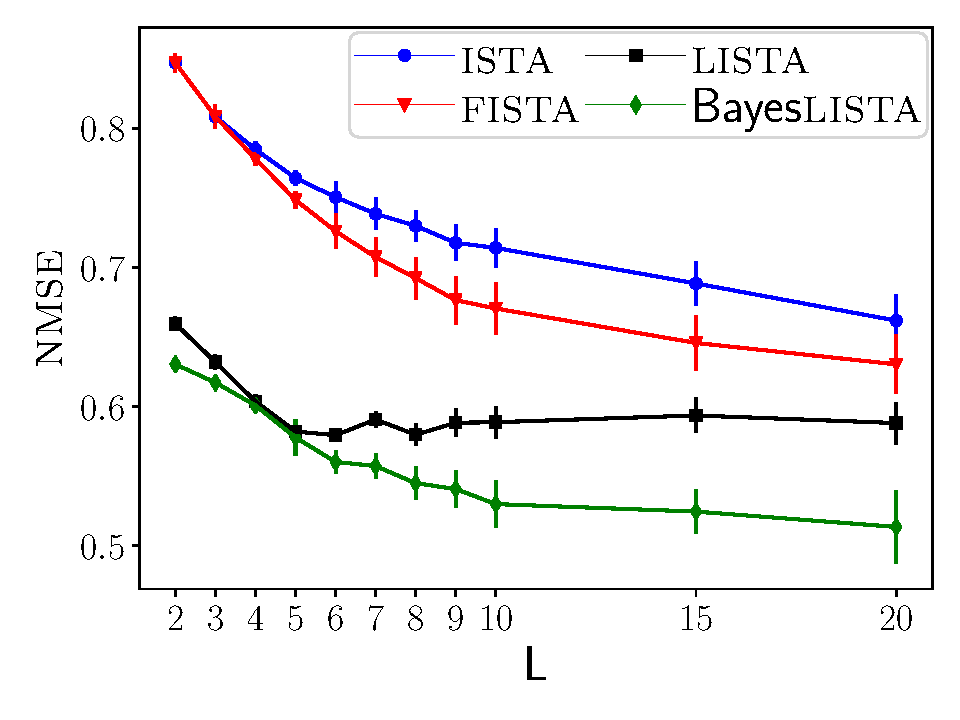
\includegraphics[width=0.24\textwidth]{graphics/synthetic_number_of_layers/nmse_validation}
  \label{fig:nmse_n_layers_synthetic}}
  \hfil
  \subfloat[Synthetic for different $K$]{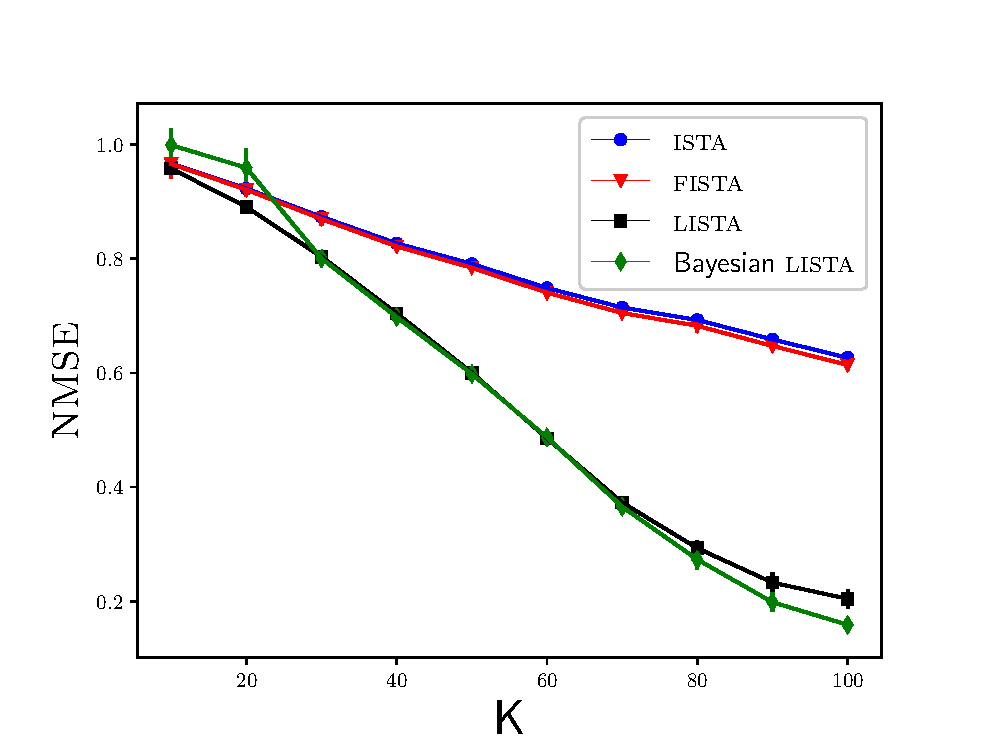
\includegraphics[width=0.24\textwidth]{graphics/synthetic_undersampling/nmse_validation}
  \label{fig:nmse_undersampling_synthetic}}
  \hfil
  \subfloat[\textsc{mnist} for $K = 100$]{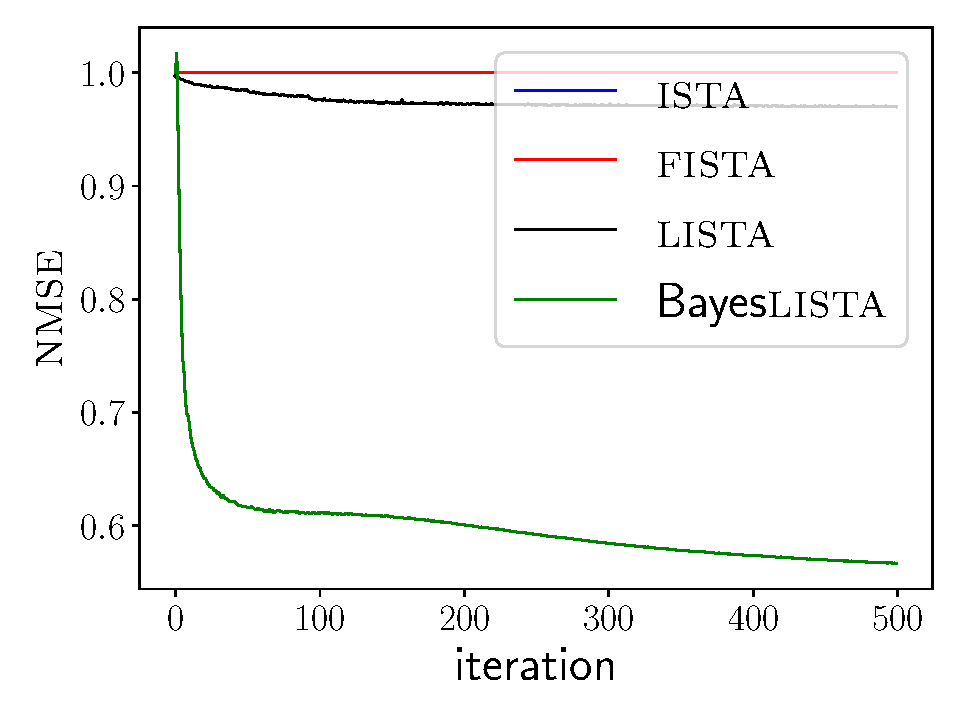
\includegraphics[width=0.24\textwidth]{graphics/mnist/100_nmse_valid}
  \label{fig:nmse_k_100}}
  \hfil
  \subfloat[\textsc{mnist} for $K = 250$]{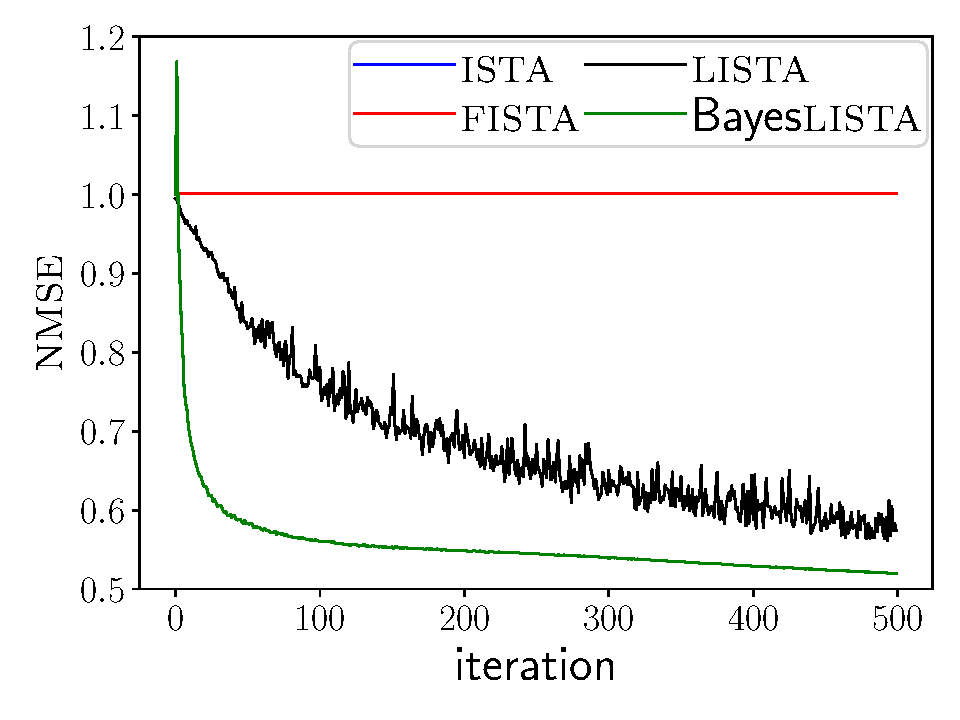
\includegraphics[width=0.24\textwidth]{graphics/mnist/250_nmse_valid}
  \label{fig:nmse_k_250}}
  \caption{\textsc{nmse} results. The synthetic data results for different number of layers~\protect\subref{fig:nmse_n_layers_synthetic} and for different sizes of observations~\protect\subref{fig:nmse_undersampling_synthetic}. The \textsc{mnist} results for increasing number of iterations with the observation size $K = 100$~\protect\subref{fig:nmse_k_100} and $K = 250$~\protect\subref{fig:nmse_k_250}}
  \label{fig:number_of_layers_synthetic}
  \end{figure*}

    \begin{figure}[!t]
  \centering
  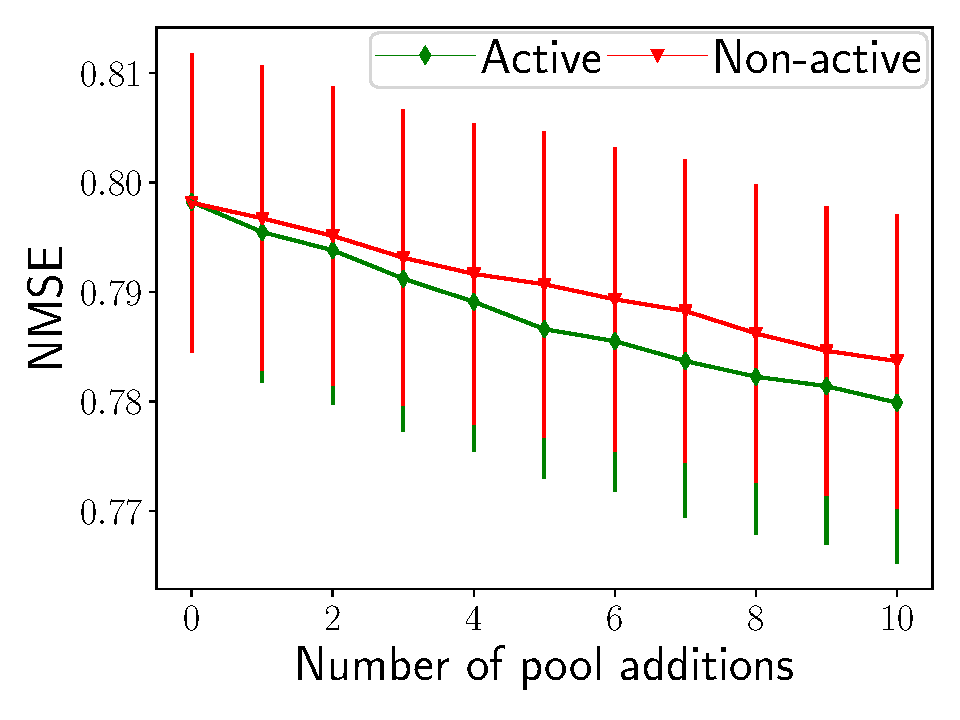
\includegraphics[width=0.24\textwidth]{graphics/active_mnist/nmse_validation}
  %\subfloat[F measure]{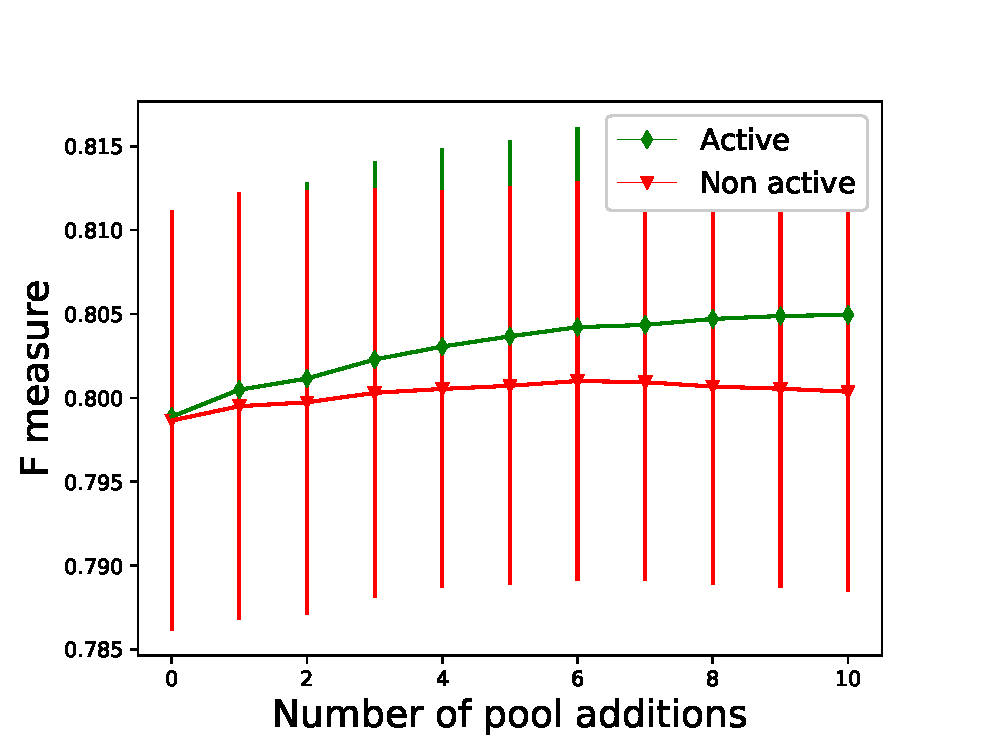
\includegraphics[width=0.48\columnwidth]{graphics/active_mnist/f_measure_validation}}
  \caption{\textsc{nmse} for the active learning experiment on \textsc{mnist} data. }
  \label{fig:active_learning_mnist}
  \end{figure}

  Proposed Bayes\textsc{lista} is evaluated on sparse coding problems and compared with \textsc{lista}~\cite{gregor2010learning}, \textsc{ista} \cite{daubechies2004iterative} and Fast \textsc{ista} (\textsc{fista}) \cite{beck2009fast}. The number of iterations in \textsc{ista} and \textsc{fista} is same as the number of layers in NNs, denoted as $L$. Quality is measured as the normalised mean square error (\textsc{nmse}). %We demonstrate the performance on small datasets to highlight that the proposed algorithm can infer accurate predictions when the dataset size is not sufficient for \textsc{lista} to learn.

  \subsection{Predictive performance on synthetic data}
  First, performance is analysed on synthetic data. We generate $N_\text{train}=1000$ and $N_{\text{test}} = 100$ sparse vectors $\boldsymbol\beta^{(n)}$ of size $D = 100$  from the spike and slab distribution with the truncated slab: each component $\beta^{(n)}_{d}$ is zero with the probability~$0.8$ or is sampled from the standard Gaussian distribution without interval $(-0.1, 0.1)$ with the probability~$0.2$. The design matrix $\mathbf{X}$ is random Gaussian.  The observations $\mathbf{y}^{(n)}$ are generated as in~(\ref{eq:regression_problem}) with the zero-mean Gaussian noise with the standard deviation $0.5$. The shrinkage parameter is set to~$\lambda = 0.1$. The algorithms are trained on the training data of size $N_\text{train}$ and evaluated on the test data of size $N_{\text{test}}$.

  In \figurename~\ref{fig:nmse_n_layers_synthetic} \textsc{nmse} for up to 20 layers (or iterations) $L$ is presented. The observation size is set to $K=50$. Bayes\textsc{lista} outperforms competitors.
%  \begin{figure}[t]
%  \centering
%  \subfloat[\textsc{nmse} on train]{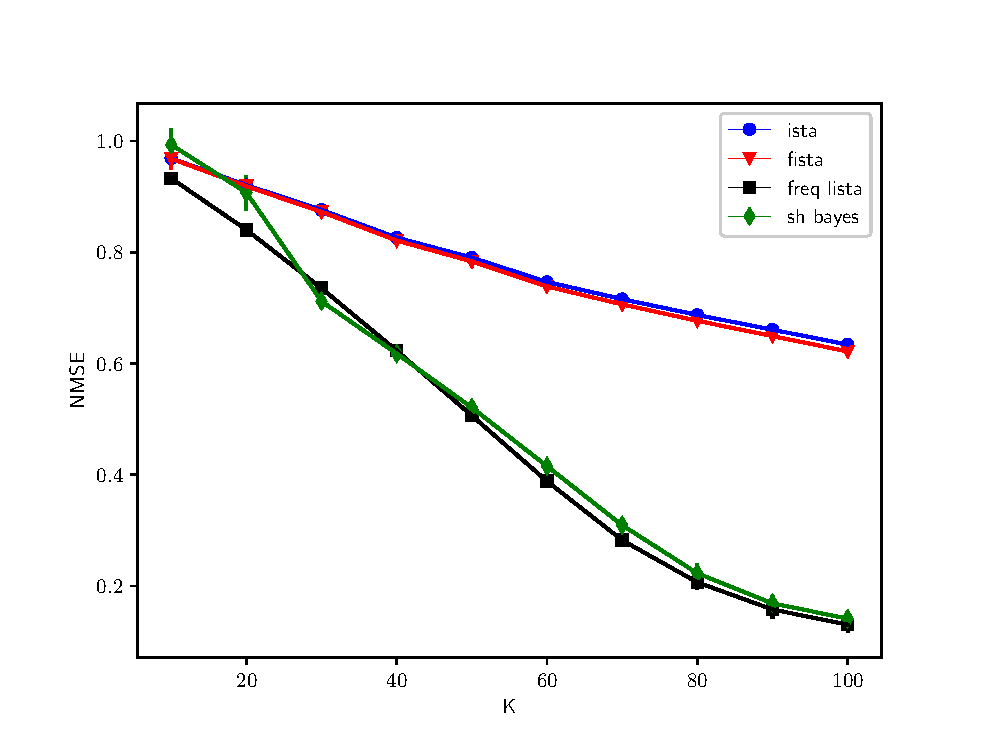
\includegraphics[width=0.5\columnwidth]{graphics/synthetic_number_of_layers/nmse_train}}
%  ~
%  \subfloat[\textsc{nmse} for different $L$]{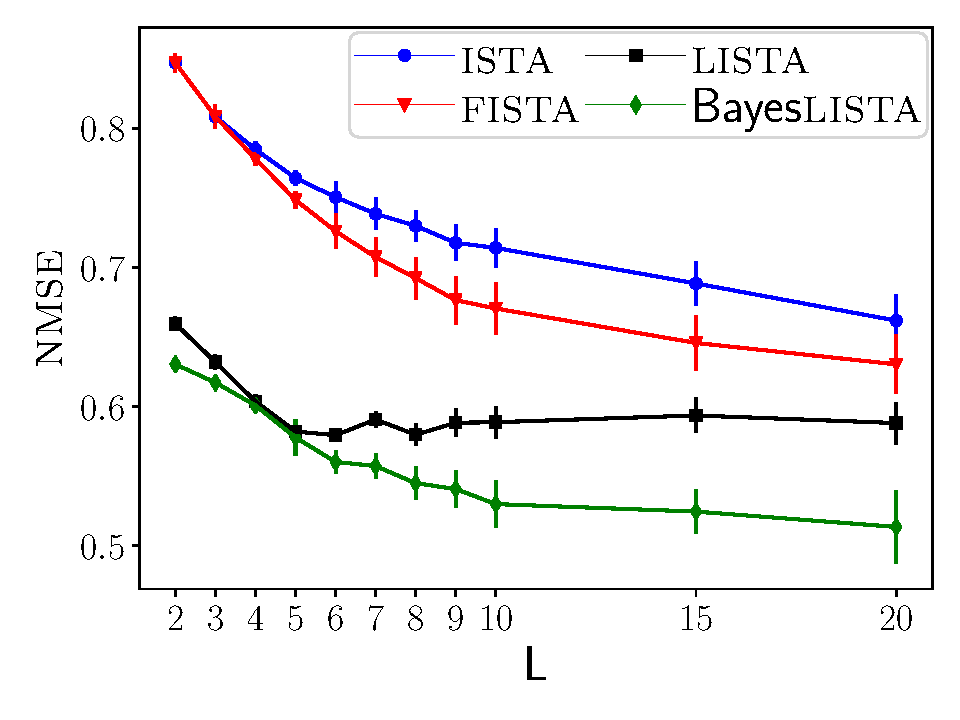
\includegraphics[width=0.48\columnwidth]{graphics/synthetic_number_of_layers/nmse_validation}
%  \label{fig:nmse_n_layers_synthetic}}
%  \subfloat[F measure on train]{\includegraphics[width=0.5\columnwidth]{graphics/synthetic_number_of_layers/f_measure_train}}
%  ~
%  \subfloat[F measure for different $L$]{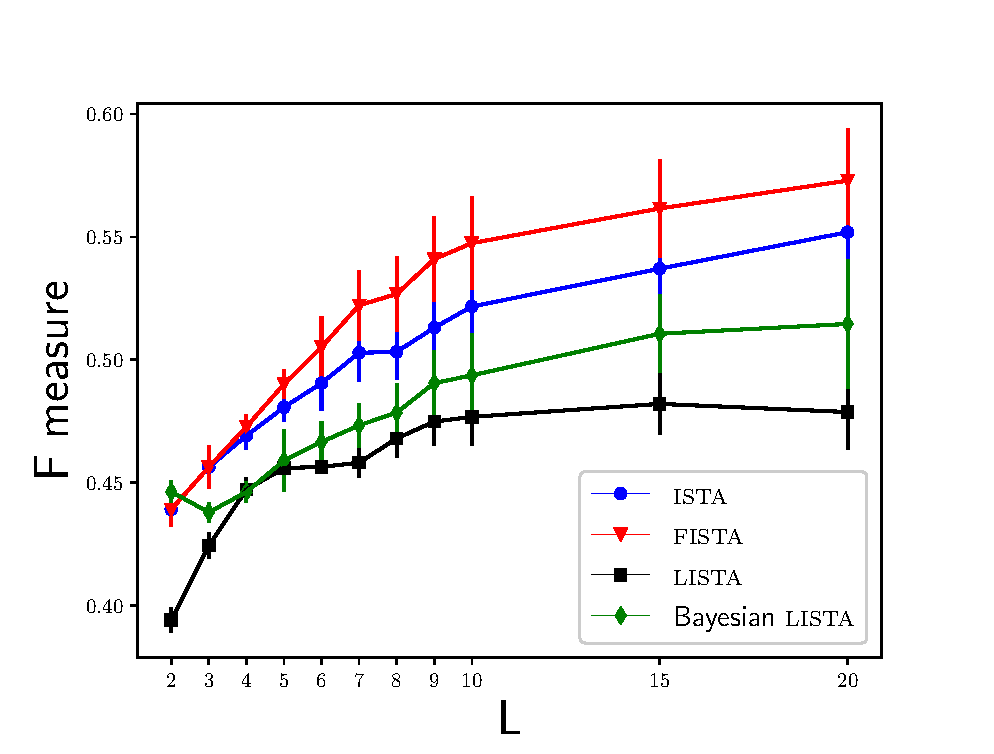
\includegraphics[width=0.48\columnwidth]{graphics/synthetic_number_of_layers/f_measure_validation}
%  \label{fig:f_meas_n_layers_synthetic}}\\[-13pt]
%  \subfloat[\textsc{nmse} for different $K$]{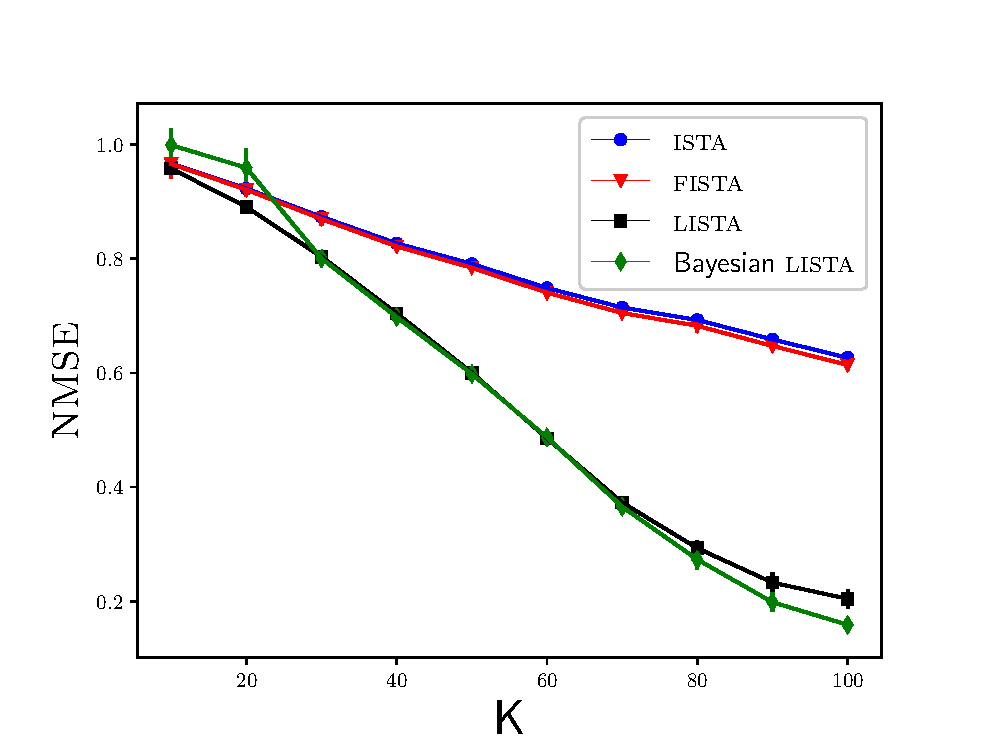
\includegraphics[width=0.48\columnwidth]{graphics/synthetic_undersampling/nmse_validation}
%  \label{fig:nmse_undersampling_synthetic}}
%  \subfloat[F measure on train]{\includegraphics[width=0.5\columnwidth]{graphics/synthetic_undersampling/f_measure_train}}
%  ~
%  \subfloat[F measure for different $K$]{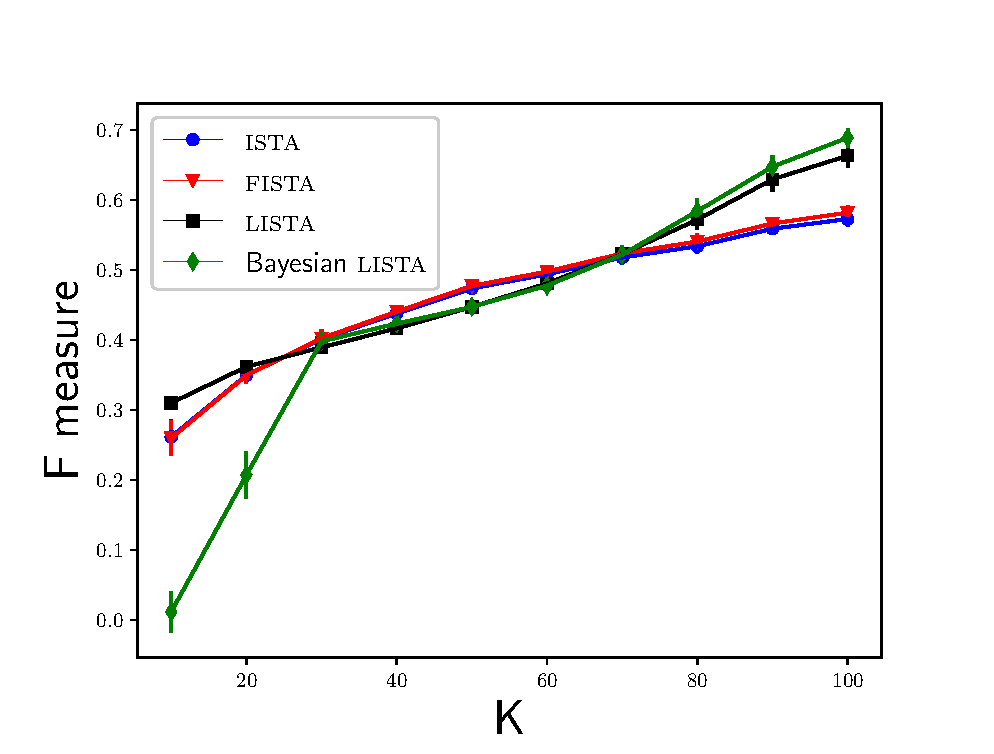
\includegraphics[width=0.48\columnwidth]{graphics/synthetic_undersampling/f_measure_validation}
%  \label{fig:f_meas_undesampling_synthetic}}
%  \caption{Predictive accuracy on the synthetic data: for different numbers of layers (for neural networks) or iterations (for baselines), and for different sizes of observations}
%  \label{fig:number_of_layers_synthetic}
%  \end{figure}
   \figurename~\ref{fig:nmse_undersampling_synthetic} gives \textsc{nmse} for different observation sizes $K$. The number of layers (iterations) is set as $L=4$. In the previous experiment, Bayesian and classic \textsc{lista} show similar results with this number of layers. \figurename~\ref{fig:nmse_undersampling_synthetic} confirms this competitive behaviour between two \textsc{lista}s. \textsc{ista} and \textsc{fista} underperform the NNs. %Overall, the experiments on the synthetic data demonstrate that Bayesian \textsc{lista} provides competitive results in terms of predictive accuracy.


  \subsection{Predictive performance on \textsc{mnist} data}
  In this experiment, the methods are evaluated on the \textsc{mnist} dataset \cite{lecun1998gradient}. The dataset contains images of handwritten digits of size $28 \times 28 = 784$. The design matrix $\mathbf{X}$ is standard random Gaussian. Observations are generated as $\mathbf{y} = \mathbf{X}\boldsymbol\beta$, where $\boldsymbol\beta \in \mathbb{R}^{784}$ are flattened images. We use $100$ images for training and $100$ for test. The shrinkage parameter $\lambda$ is~$0.1$.

  Figures \ref{fig:nmse_k_100} and~\ref{fig:nmse_k_250} present \textsc{nmse} with observation sizes $100$ and $250$. The experiment with $K=100$ presents severe conditions for the algorithms: the limited size of the training dataset combined with the small dimensionality of observations. Bayes\textsc{lista} is able to learn under these conditions, significantly outperforming \textsc{lista}. Under better conditions of the second experiment with $K=250$, both NNs converge to the similar results. However, Bayes\textsc{lista} demonstrates a remarkably better convergence rate. \textsc{ista} and \textsc{fista} are unable to perform well in these experiments.

%  \begin{figure}[t!]
%  \centering
%  %\subfloat[\textsc{nmse} on train]{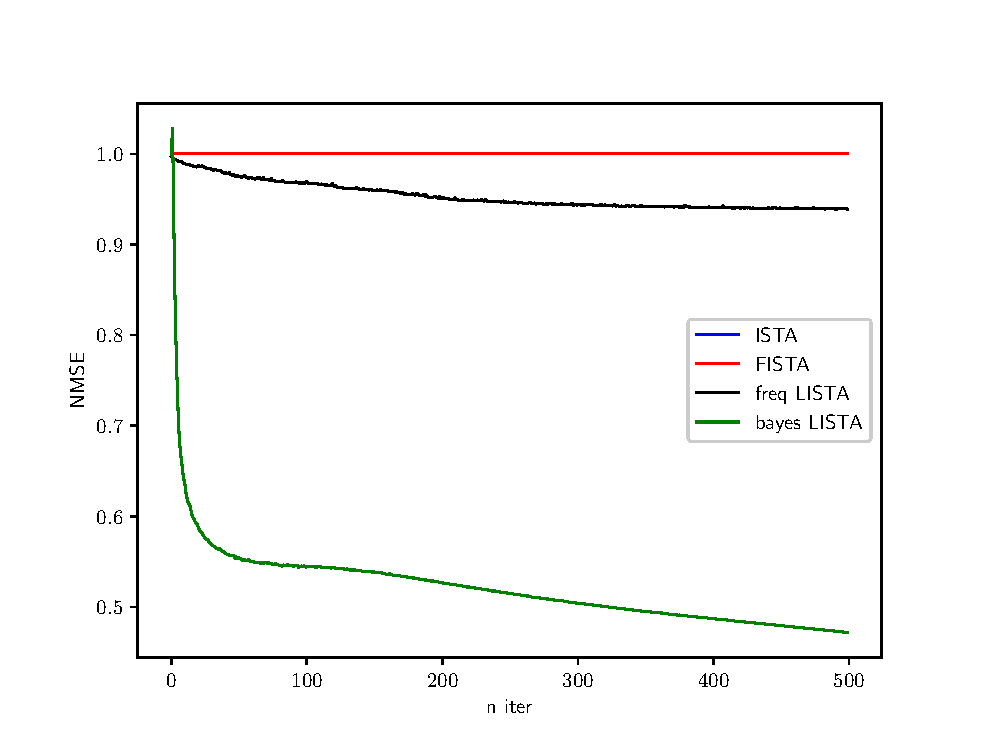
\includegraphics[width=0.5\columnwidth]{graphics/mnist/100_normalised_nmse_train}}
%  %~
%  \subfloat[\textsc{nmse} for $K = 100$]{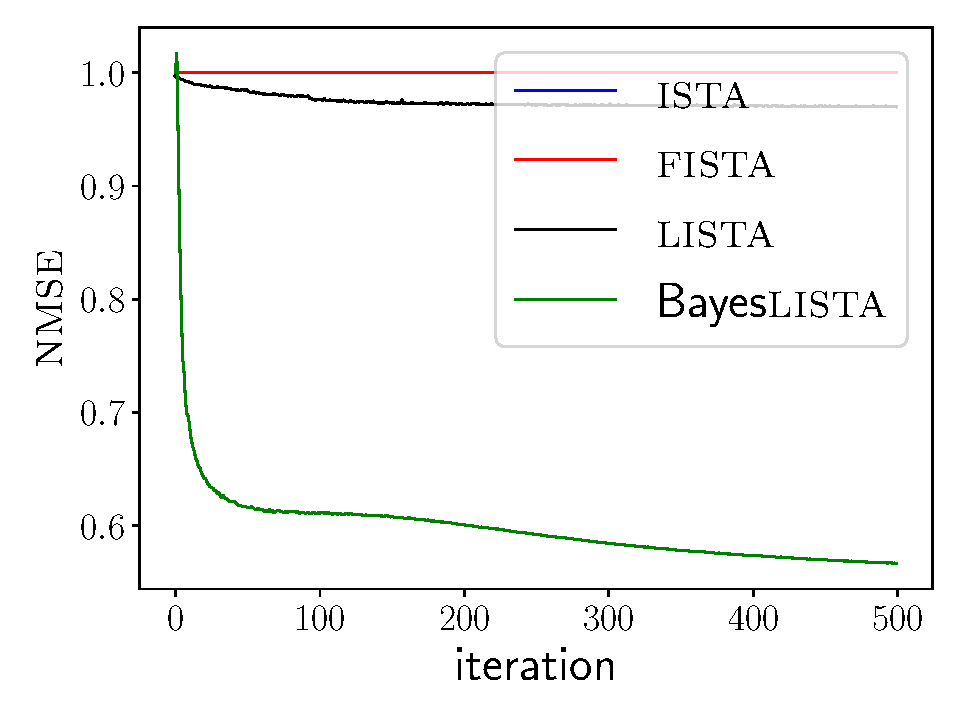
\includegraphics[width=0.48\columnwidth]{graphics/mnist/100_nmse_valid}}
%  %\subfloat[F measure on train]{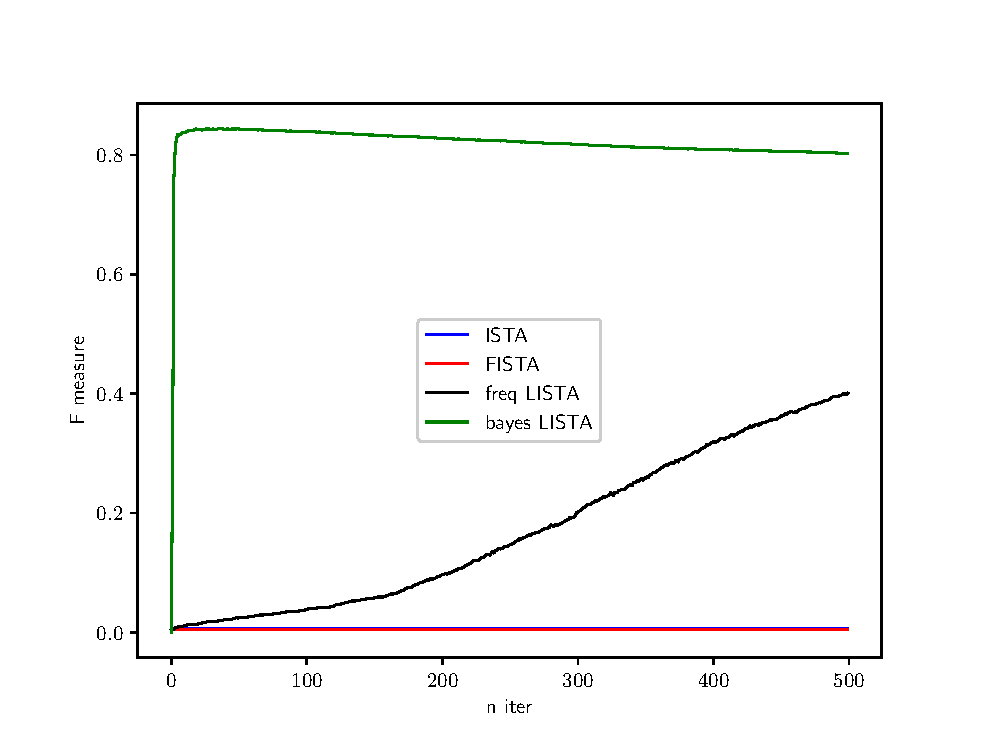
\includegraphics[width=0.5\columnwidth]{graphics/mnist/100_normalised_f_measure_train}}
%  %~
%  %\subfloat[F measure for $K = 100$]{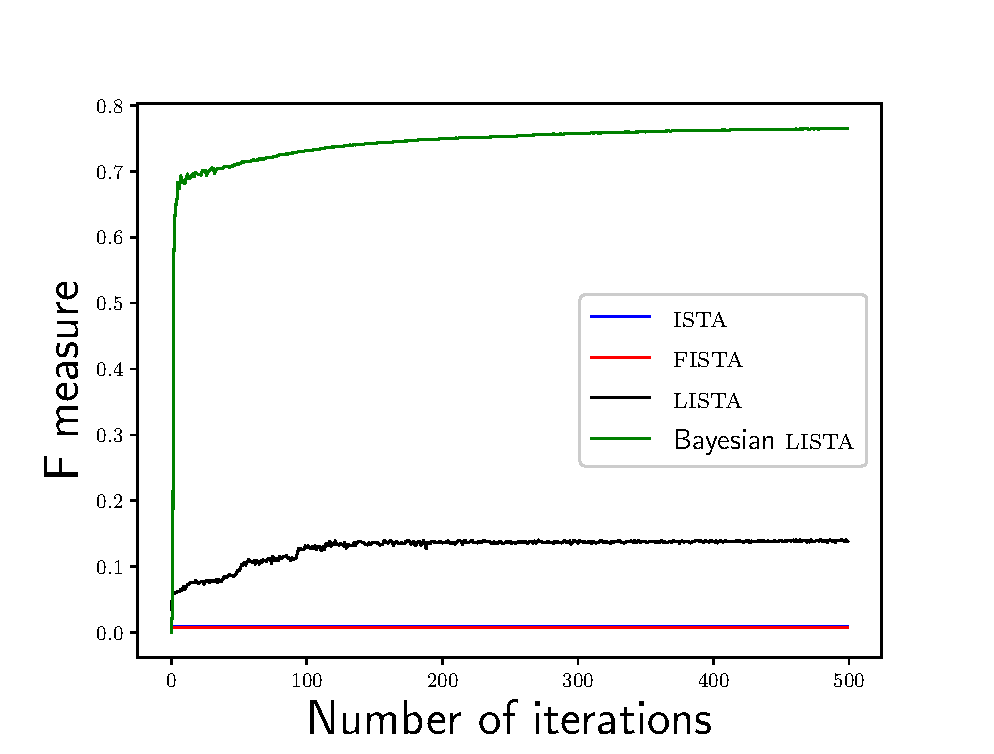
\includegraphics[width=0.48\columnwidth]{graphics/mnist/100_f_measure_valid}}\\[-13pt]
%  \subfloat[\textsc{nmse} for $K = 250$]{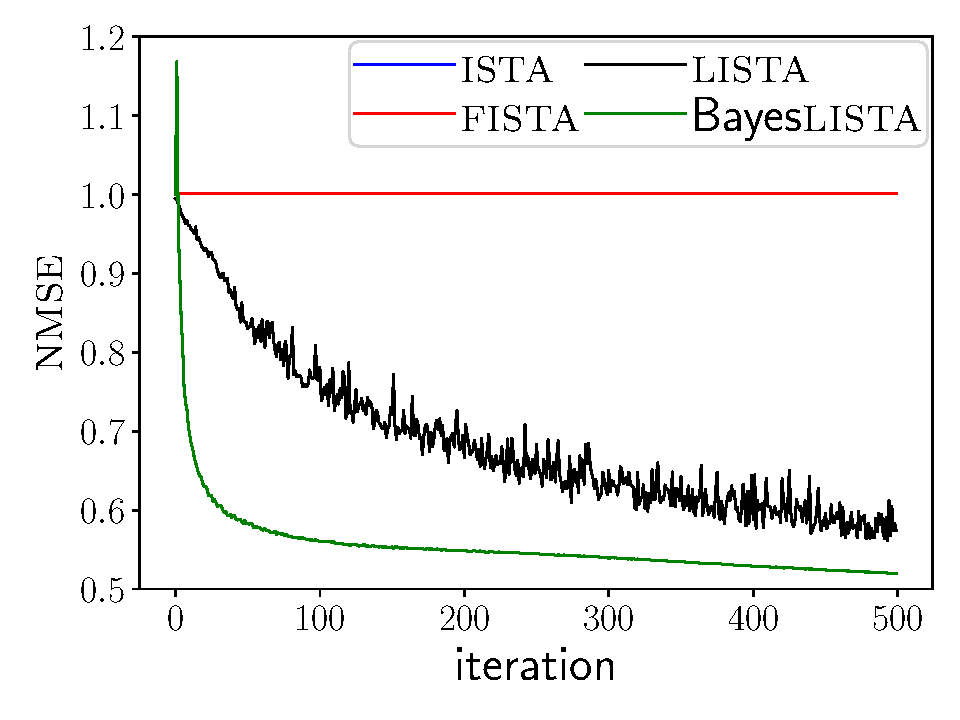
\includegraphics[width=0.48\columnwidth]{graphics/mnist/250_nmse_valid}}
%  %\subfloat[F measure on train]{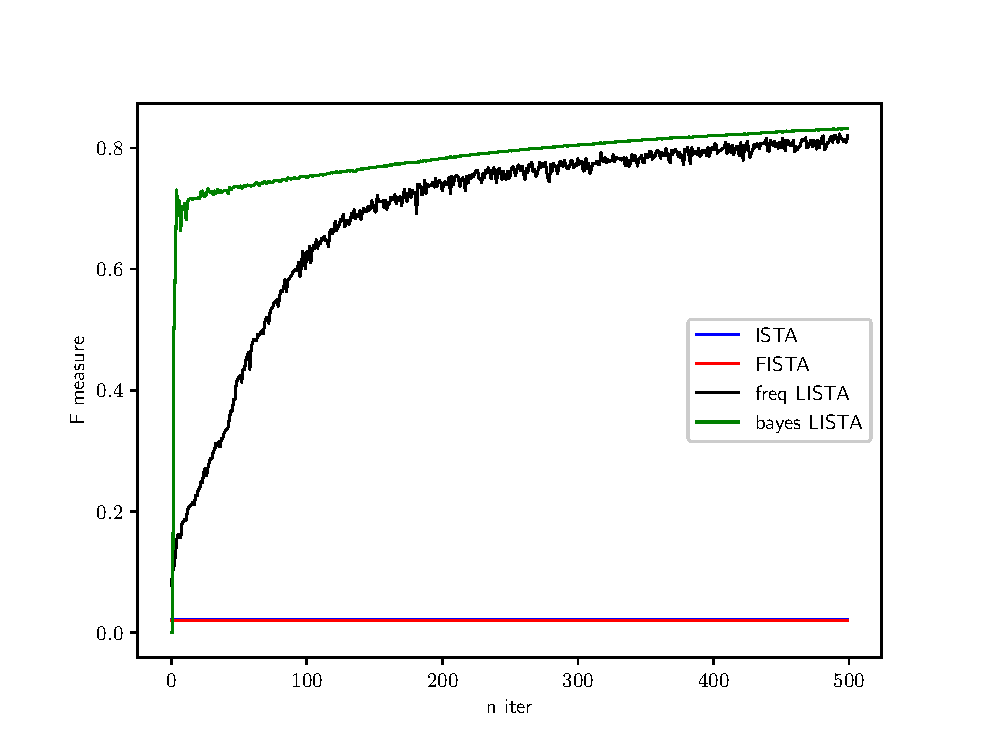
\includegraphics[width=0.5\columnwidth]{graphics/mnist/250_normalised_f_measure_train}}
%  %~
%  %\subfloat[F measure for $K = 250$]{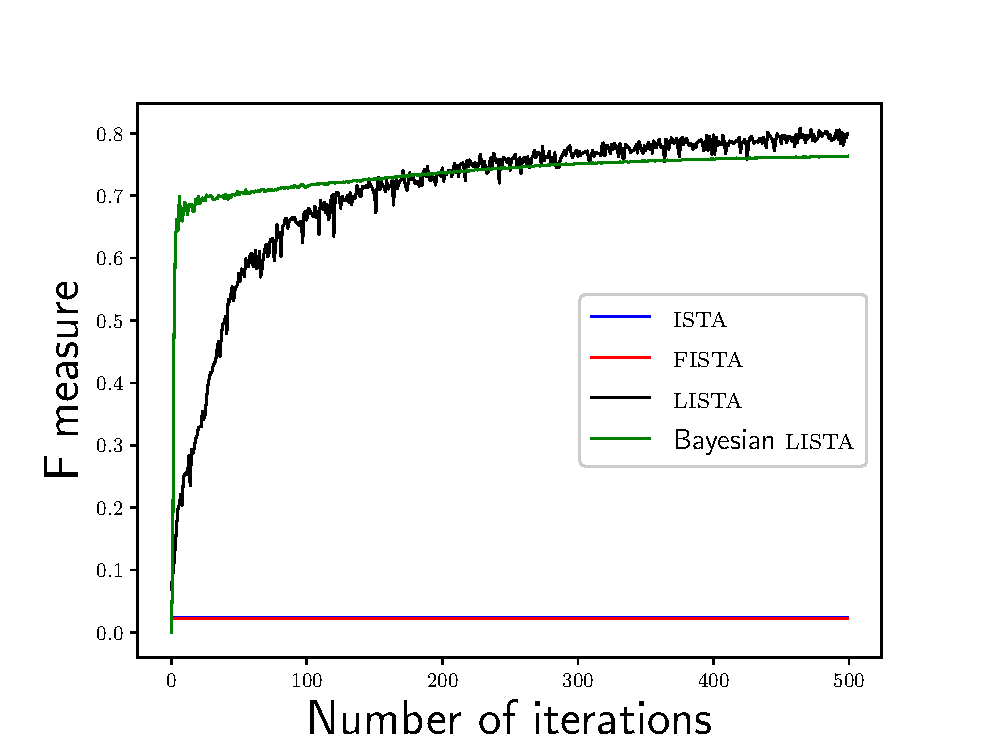
\includegraphics[width=0.48\columnwidth]{graphics/mnist/250_f_measure_valid}}
%  \caption{Predictive performance for different numbers of iterations on the \textsc{mnist} data with the observation size $K = 100$ and $K = 250$}
%  \label{fig:mnist}
%  \end{figure}

  \subsection{Active learning}
  To demonstrate a potential scenario that can benefit from uncertainty estimates of Bayes\textsc{lista}, we consider the active learning example~\cite{settles.tr09}. The active learning area researches ways to select new training subsets to reduce the total number of required supervision. One of the popular approaches in active learning is uncertainty sampling, when the data with the least certain predictions is chosen for labelling. We use a variance (\ref{eq:spsl_moments}) as a measure of uncertainty.

 The \textsc{mnist} dataset with the observation size $K=100$ is utilised. We use the training data of size $50$, the pool data of size $500$,  and the test data of size $100$. The algorithm learns on the training data and it is evaluated on the test data. To actively collect a next data point from the pool, the algorithm is used to predict a point with the highest uncertainty. The selected point is moved from the pool to the training data and the algorithms learns on the updated training data. Overall, $10$ pool additions are performed. After every addition the performance is measured on the test data. We compare the active approach of adding new points from the pool with the random approach that picks a new data point from the pool at random. The procedure is repeated for $20$ times.

  Figure \ref{fig:active_learning_mnist} demonstrates performance of the active and non-active methods of updates with Bayes\textsc{lista}. The active approach with uncertainty sampling steadily demonstrates better results. This means the posterior distribution learnt by Bayes\textsc{lista} is an adequate estimate of the true posterior.

  \section{Conclusions}
  \label{sec:conclusions}
 % To the best of our knowledge, this is the first implementation of a Bayesian deep sparse coding algorithm. %Although there are works on Bayesian sparsity in context of neural networks \cite{he2017bayesian}, they are not the Bayesian neural networks in the same sense as Bayesian \textsc{lista} but rather the interpretation of the sparse Bayesian  learning algorithm as the long short-term memory network. We find not only correct predictions but also useful posterior estimates for the predictions.
  We have presented the new method for propagating uncertainty through the soft-thresholding function.
  %We have approximated the outputs of the function with a spike and slab distribution, and we have shown that this distribution can stay within the same family after linear transformation with Gaussian weights and inputs of a neural network.
  This allowed us to propose Bayes\textsc{lista} and efficient inference algorithm that learns the distributions of the weights and makes the uncertainty estimates of the outputs. %The forward propagation in the algorithm is based on the proposed uncertainty propagation method, the backward propagation is based on the probabilistic backpropagation method, that was remarkably expanded to account for multidimensionality of inputs and outputs, likelihood of Bayesian \textsc{lista} and its recurrent nature.

%  Experiments on the synthetic and \textsc{mnist} datasets demonstrate that the proposed algorithm preserves the predictive accuracy of non-Bayesian methods while also providing posterior estimates. We also show that when the training data is very small the proposed algorithm significantly outperforms \textsc{lista} in terms of predictive accuracy. Active learning experiments demonstrate that Bayes\textsc{lista} gives accurate posterior estimates that can be used to select new training data points.



% Below is an example of how to insert images. Delete the ``\vspace'' line,
% uncomment the preceding line ``\centerline...'' and replace ``imageX.ps''
% with a suitable PostScript file name.
% -------------------------------------------------------------------------
% \begin{figure}[htb]

% \begin{minipage}[b]{1.0\linewidth}
%   \centering
%   \centerline{\includegraphics[width=8.5cm]{image1}}
% %  \vspace{2.0cm}
%   \centerline{(a) Result 1}\medskip
% \end{minipage}
% %
% \begin{minipage}[b]{.48\linewidth}
%   \centering
%   \centerline{\includegraphics[width=4.0cm]{image3}}
% %  \vspace{1.5cm}
%   \centerline{(b) Results 3}\medskip
% \end{minipage}
% \hfill
% \begin{minipage}[b]{0.48\linewidth}
%   \centering
%   \centerline{\includegraphics[width=4.0cm]{image4}}
% %  \vspace{1.5cm}
%   \centerline{(c) Result 4}\medskip
% \end{minipage}
% %
% \caption{Example of placing a figure with experimental results.}
% \label{fig:res}
% %
% \end{figure}


% % To start a new column (but not a new page) and help balance the last-page
% % column length use \vfill\pagebreak.
% % -------------------------------------------------------------------------
% %\vfill
% %\pagebreak

% \section{COPYRIGHT FORMS}
% \label{sec:copyright}

% You must submit your fully completed, signed IEEE electronic copyright release
% form when you submit your paper. We {\bf must} have this form before your paper
% can be published in the proceedings.

% \section{RELATION TO PRIOR WORK}
% \label{sec:prior}

% The text of the paper should contain discussions on how the paper's
% contributions are related to prior work in the field. It is important
% to put new work in  context, to give credit to foundational work, and
% to provide details associated with the previous work that have appeared
% in the literature. This discussion may be a separate, numbered section
% or it may appear elsewhere in the body of the manuscript, but it must
% be present.

% You should differentiate what is new and how your work expands on
% or takes a different path from the prior studies. An example might
% read something to the effect: "The work presented here has focused
% on the formulation of the ABC algorithm, which takes advantage of
% non-uniform time-frequency domain analysis of data. The work by
% Smith and Cohen \cite{Lamp86} considers only fixed time-domain analysis and
% the work by Jones et al \cite{C2} takes a different approach based on
% fixed frequency partitioning. While the present study is related
% to recent approaches in time-frequency analysis [3-5], it capitalizes
% on a new feature space, which was not considered in these earlier
% studies."

% \vfill\pagebreak

% \section{REFERENCES}
% \label{sec:refs}

% List and number all bibliographical references at the end of the
% paper. The references can be numbered in alphabetic order or in
% order of appearance in the document. When referring to them in
% the text, type the corresponding reference number in square
% brackets as shown at the end of this sentence \cite{C2}. An
% additional final page (the fifth page, in most cases) is
% allowed, but must contain only references to the prior
% literature.

% % References should be produced using the bibtex program from suitable
% % BiBTeX files (here: strings, refs, manuals). The IEEEbib.bst bibliography
% % style file from IEEE produces unsorted bibliography list.
% % -------------------------------------------------------------------------
\bibliographystyle{IEEEbib}
\bibliography{bibliography}

\end{document}
